\documentclass[11pt]{article}
\usepackage[english,russian]{babel}
\usepackage{url}
\usepackage{graphicx,DCCN2021_ru}

\pagestyle{fancy} 
\fancyhead{} 
\fancyfoot{} 

\usepackage[utf8]{inputenc}
\linespread{1.0}

\usepackage{amsmath}
% Название доклада на русском языке:
\title{ИСПОЛЬЗОВАНИЕ ГЕНЕТИЧЕСКИХ АЛГОРИТМОВ ПРИ ОПТИМИЗАЦИИ СТРАТЕГИЙ ИГР С НЕПОЛНОЙ ИНФОРМАЦИЕЙ НА ПРИМЕРЕ ИГРЫ «ДОМИНО»}

\author{\small \textbf{Шанин Р.Е.}}
%Аффилиация авторов
\affil{\footnotesize РТУ-МИРЭА, проспект Вернадского, 78, г.Москва, Россия}

\email{shanin1000@yandex.ru}
%%%%%%%%%%%%%%%%%%%%%%%%%%%%%%%%
\begin{document}
\udk{004.09}
{\let\newpage\relax\maketitle}
%\maketitle
\vskip -1.5em

% Аннотация
%%%%%%%%%%%%%%%%%%%%%%%%%%%%%%%%%%%%%%%%%%%%%%%%%%%%%%%%%%%%%%
\begin{abstract}
В работе рассмотрен подход к созданию системы искусственного интеллекта на примере игры «Домино». Применен генетический алгоритм для оптимизации стратегии игры. Выполнен сравнительный анализ реализованных подходов для определения эффективности оптимизации игровых стратегий с помощью генетических алгоритмов.
\keywords{генетические алгоритмы, искусственный интеллект, игры с неполной информацией, игра «Домино»}
\end{abstract}
%%%%%%%%%%%%%%%%%%%%%%%%%%%%%%%%%%%%%%%%%%%%%%%%%%%%%%%%%%%%%%
\section{Введение}
Введение. В последние годы наблюдается тренд на создания систем искусственного интеллекта, действующих в условиях неопределённости реального мира. В качестве примера моделирования такой неопределенности можно рассмотреть широко известную игру «Домино». «Домино» – игра, в которой игрокам неизвестно полное состояние игры, также игра «Домино» обладает простыми правилами, которые формализуются достаточно просто. Например, в работе \cite{bib2} рассмотрен алгоритм принятия решения, основанный на деревьях решений. При таком подходе поведение системы описывается логическими блоками, принимающими решения относительно той или иной игровой ситуации. При этом за обучаемость системы отвечает блок наблюдений, который в процессе игры пытается составить вероятностное распределение камней у противника. Достоинством системы является эффективное обыгрывание типовых ситуаций, возникающих по ходу игры. Из недостатков можно выделить то, что алгоритм не предусматривает то, что среда (правила игры), в которой действует алгоритм, могут меняться. Изменение среды вызовет необходимость переписывать некоторые из логических блоков. В статье \cite{bib3} проанализированы подходы, основанные на правиле Минимакс и Perfect Information Monte Carlo (PIMC). 
{\newpage}
При таком подходе игра с неполной информацией разбивается на множество игр с полной информацией, затем для каждой игры из множества находится оптимальное действие с помощью минимакс поиска. Решением для игры с неполной информацией будет действие, найденное как взвешенные вероятностями наступления той или иной игровой ситуации решения игр с полной информацией. Для качественного принятия решений такой алгоритм требует значительных вычислительных мощностей (алгоритм перебирает множество вариантов развития игры на несколько ходов вперед). Так же в реализации предложенной в статье не предусмотрена возможность дообучения алгоритма на основе опыта игры. В данной статье предложен подход к созданию системы принятия решений для игры «Домино», основанный на эвристическом методе, который позволяет легко модифицировать систему при изменении среды, а также предусматривает обучение алгоритма при получении опыта.
    Рассмотрим вариант игры «Домино» для двух игроков и определим правила следующим образом. 

\section{Правила игры}
Рассматривается вариант игры в домино на двух игроков. В игре имеется набор S из 28 уникальных камней s, где $s_ij=(i,j), 0\leqslant i,j \leqslant6$.
В начале каждого раунда игрокам случайным образом раздается по 7 камней, остальные камни остаются в резерве. Каждый ход, начиная с первого игрока, игроки совершают одно из двух действий:
\begin{enumerate}
    \item Положить на игровое поле один из доступных камней.
    \item Брать камни из резерва по одному до тех пор, пока не появится доступный для хода камень. 
\end{enumerate}


Камень считается доступным для хода, если это первый камень, который будет выложен, или на хотя бы одном конце игрового поля число совпадает с числом на камне. Раунд заканчивается, как только у одного игрока заканчиваются камни или дальнейший ход игры не возможен. За каждый раунд игрокам присуждаются очки. Побеждает тот, кто наберет первым больше 100 очков.

\section{Постановка задачи}
Разработать алгоритм, которому дается набор доступных для хода камней, а также сведенья об игровом поле, сыгранных камнях и камнях в руке. Алгоритм должен найти оптимальный ход, ведущий к победе. Выполнить модификацию разработанного алгоритма для применения генетического алгоритма оптимизации. Сравнить полученные оптимизированные и не оптимизированные стратегии с жадным алгоритмом игры для определения эффективности оптимизации. 


\section{Алгоритм}
В качестве алгоритма, принимающего решение о выборе хода, был выбран подход на основе полезности. При таком подходе имеется некоторая функция $utilityFunc:S_ turn \times E \rightarrow \mathbb{R}$, где $S_ turn$ - множество камней доступных для хода,$E$ - множество состояний игры, которая определяет ценность хода тем или иным камнем. Когда алгоритму приходит на вход множество доступных для хода камней он вычисляет значение функции для каждого из них и выбирает камень с наибольшей ценностью. Преимуществами подхода является его компактность и легкая модификация в случае изменения среды, из недостатков можно выделить чувствительность алгоритма к выбору $utilityFunc$.


На основе опыта игры в «Домино» в качестве utilityFunc была выбрана функция, отражающая три пути достижения победы: 
\begin{enumerate}
    \item Снижение суммарного количества очков на камнях в руке, данный подход смягчает последствия поражения. 
    \item Увеличение вероятности того, что в руке противника не окажется нужного камня для совершения хода, подход ведет к увеличению суммарного количества очков в руках противника, то есть делает победы более значительными. Так же это необходимый подход, если игрок начинает вторым для перехвата инициативы. 
    \item Увеличение вероятности совершения своего следующего хода, ведет к большой вариативности проистечения партии и сохранению инициативы.
\end{enumerate}


Таким образом:
\[utilityFunc(s_{ij},e)=\frac{score(s_{ij})}{12}+p_{noturn}(s_{ij}|e)+p_{nextturn}(s_{ij}|e),\] где e – текущее состояние игры, $score(s_{ij})$– количество очков на камне $(i+j)$, $p_{noturn}(s_{ij}|e)$– вероятность того, что среди камней противника нет подходящих, $p_{nextturn}(s_{ij}|e)$ -вероятность совершить следующий ход. Все три члена суммы находятся в промежутке $[0,1]$.

\section{Оптимизация}
Следующим этапом стала оптимизация $utilityFunc$ для увеличения эффективности выбора ходов. В качестве алгоритма оптимизации был выбран генетический алгоритм (ГА). Согласно \cite{bib1}, генетические алгоритмы обладают следующими достоинствами: не требуют никакой информации о поведении функции (дифференцируемости и непрерывности) и просты в реализации.
Для применения ГА внесем следующие изменения в функцию $utilityFunc$:
\[utilityFunc(s_{ij},e)=a_1 \frac{score(s_{ij})}{12}+1_2p_{noturn}(s_{ij}|e)+a_3p_{nextturn}(s_{ij}|e),\] где вектор $a = (a_1, a_2, a_3)$ представляет стратегию игры.
Реализация генетического алгоритма включает в себя несколько этапов: 
\begin{itemize}
    \item Генерация стартового набора стратегий c количеством стратегий $k$.
    \item Отбор наиболее успешных стратегий. Отбор происходил в форме турнира, где каждая стратегия играет по одной партии против всех остальных стратегий. Сумма очков, набранная за турнир, является показателем успешности стратегии. Пример результатов предоставлен в таблице 1.
    \begin{table}[h!]\begin{center}\caption{Пример результатов турнира.}
        \begin{tabular}{|c|c|c|c|c|}\hline
          1 & 11 & 12 & 33 & 34 \\ \hline 
          11 & 00 & 778 & 338 & 1101 \\ \hline
          22 & 1103 & 00 & 1112 & 1119 \\ \hline
          33 & 1112 & 223 & 00 & 996 \\ \hline
          44 & 772 & 558 & 1154 & 00 \\ \hline
        \end{tabular}\label{tab:result example}
        \end{center}\end{table}
\item Стратегии сортируются по своей успешности. Стратегии оказавшееся в половине наименее успешных стратегий отсекаются.
\item Начальное количество стратегий восстанавливается благодаря смешению существующих успешных стратегий. Выбираются две стратегии $a=(a_1,a_2,a_3)$ и $b=(b_1,b_2,b_3)$. Новой стратегией будет стратегия $c$, где $c_i$  выбирается случайно из $(a_i,b_i,\frac{a_i+b_i}{2},0)$ После чего, с некоторой вероятностью $p$, $c_i$ может подвергнуться небольшому случайному изменению.
\end{itemize}


Описанные шаги повторяются пока n повторений подряд схожие стратегии не будут самыми успешными. Схожесть определяется как $\|a-b\|^2<\epsilon$, где $\epsilon$ некоторая константа.

В ходе применения ГА было обнаружено несколько проблем: 
При реализации турнира как все против всех время, требуемое на проведения турнира, растет как $O(n^2)$ от количества стратегий в стартовом наборе.
В некоторых случаях в ходе оптимизации стратегии в наборе вырождаются и представляют одну или набор близких стратегий.
Реализация и сравнительный анализ. На основе изложенного выше подхода была реализована программа средствами языка Python. В программе предусмотрен консольный интерфейс элементы, которого представлены на рисунке 1.

{\newpage}
\begin{figure}
    \centering
    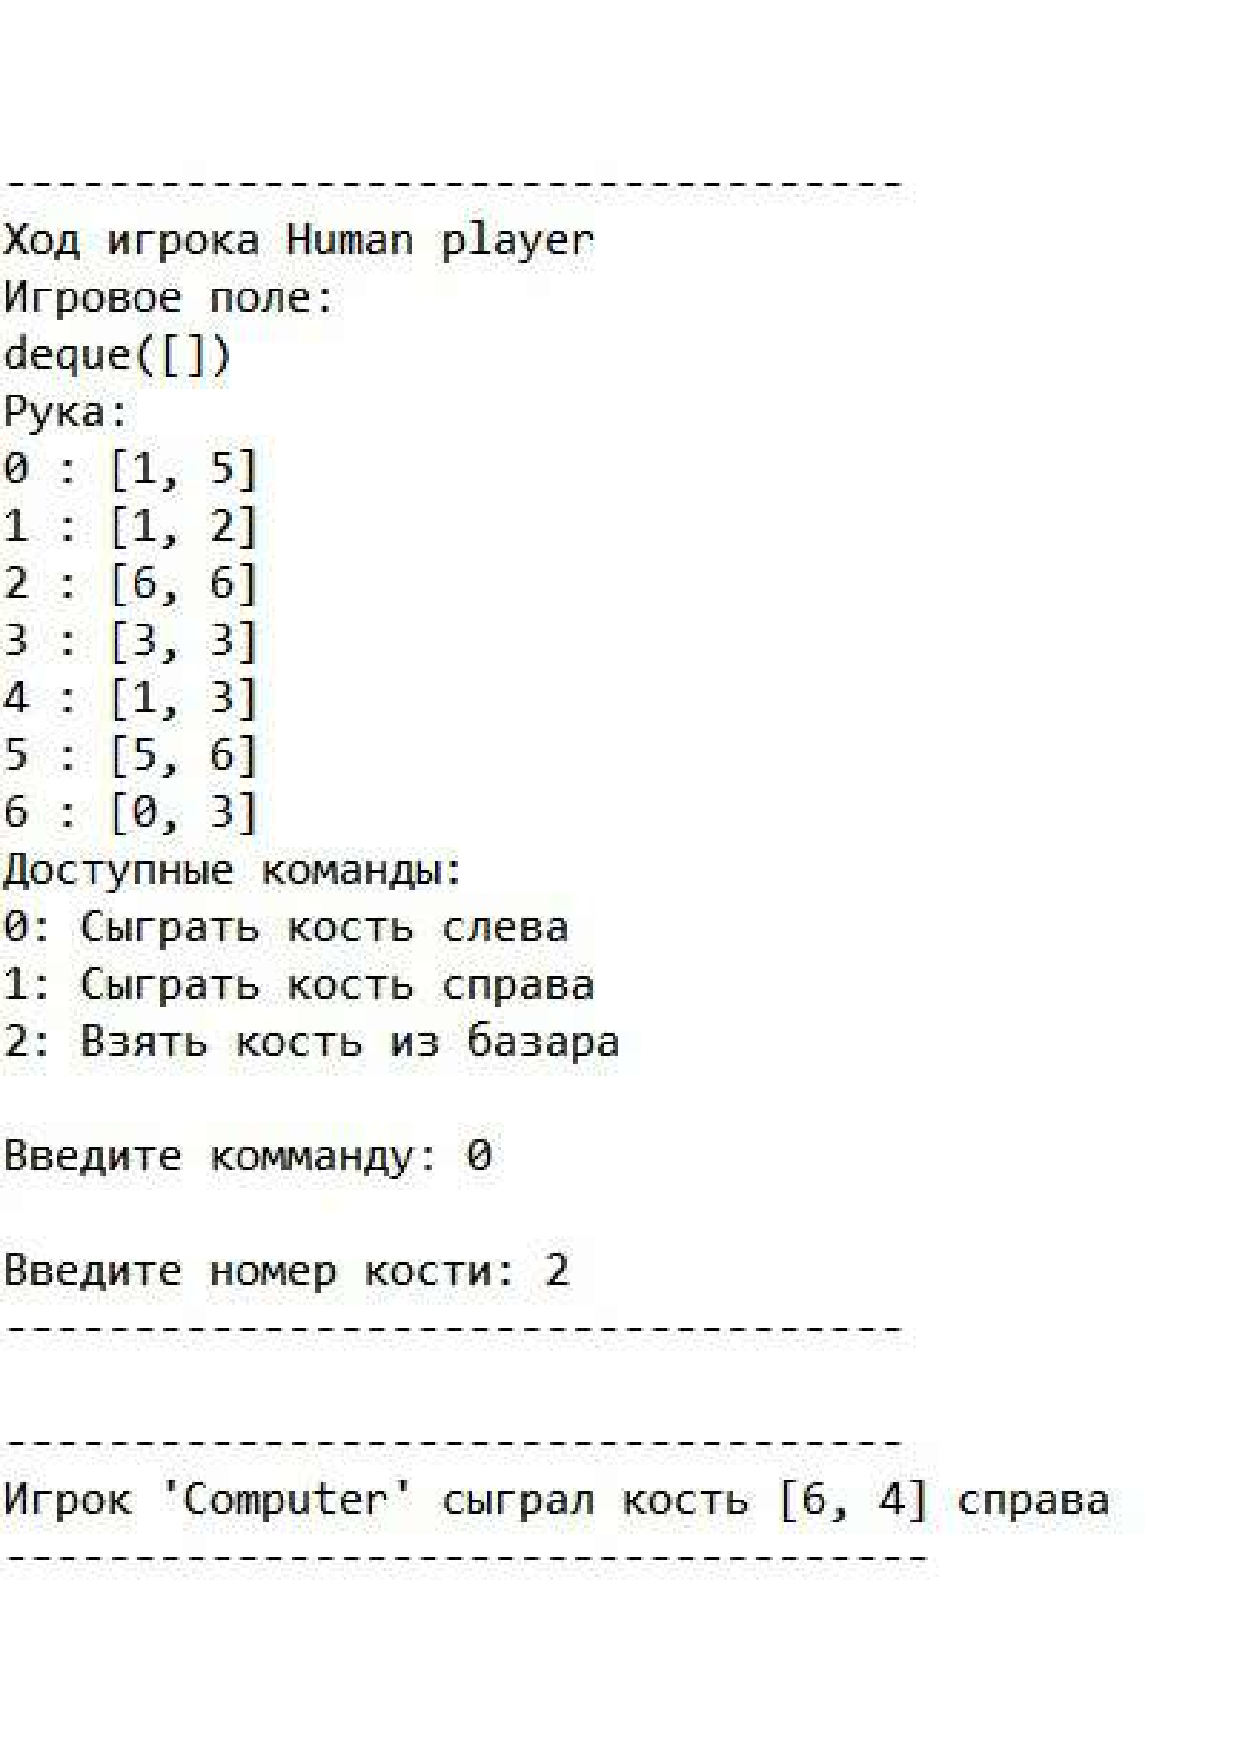
\includegraphics[width=0.5\textwidth]{DOMINO.pdf}
    \caption{\label{fig:consoleapplicationview}Вид консольного интерфейса приложения.}
  \end{figure}

С помощью реализованной программы был проведен сравнительный анализ различных игровых стратегий. В качестве стратегии для сравнения была выбран жадная стратегия игры в «Домино». Сначала была протестирована неоптимизированная стратегия, после чего были протестированы оптимизированные стратегии с различными параметрами оптимизации. Для оценки результатов были проведены 1000 игр до 100 очков. Результаты предоставлены в таблице 2. 

\begin{table}[h!]\begin{center}\caption{Сравнительный анализ различных стратегий.}
\begin{tabular}{|c|c|c|}\hline
  Стратегия & Побед & Поражений  \\ \hline 
  Неоптимизированная & 831 & 179 \\ \hline
  Оптимизированная $(0.0, 1.0, 0.0)$ & 845 & 155 \\ \hline
  Оптимизированная $(0.17, 1.0, 0.2)$ & 866 & 134 \\ \hline
\end{tabular}\label{tab:comparing strategy analyze}
\end{center}\end{table}

Из результатов сравнительного анализа видно, что проведение оптимизации привело лишь к небольшому улучшению соотношения побед/поражений. Это может быть связанно с несколькими причинами: 
\begin{enumerate}
    \item На исход партии влияет не только оценочная способность алгоритма, но и начальная раздача камней. Таким образом стратегии достигают предела при, котором дальнейшее увеличение соотношение процента побед затруднено в силу неблагоприятных начальных условий.
    \item Способность оценки функции полезности слабо зависит от стратегии.
    \item Неоптимизированная стратегия $(1, 1, 1)$ близка к оптимальной.
\end{enumerate}
 Для проверки приведенных выше предположений была проведена новая серия тестов, в которой стратегии сравнивались с начальной неоптимизированной стратегией $(1,1,1)$. Так же для проверки предположения 3 было введено сравнение со случайной стратегией. Результаты приведены в таблице 3.

\begin{table}[h!]
\begin{center}\caption{Дополнительные тестирования стратегий.}
\begin{tabular}{|c|c|c|}\hline
    Стратегия & Побед & Поражений  \\ \hline 
    Случайная стратегия & 392 & 608 \\ \hline
    Оптимизированная $(0.0, 1.0, 0.0)$ & 521 & 479 \\ \hline
    Оптимизированная $(0.17, 1.0, 0.2)$ & 574 & 426 \\ \hline
\end{tabular}\label{tab:extended testing of strategy}
\end{center}\end{table}

На основе этого анализа можно сделать вывод, что предположение 2 не верно, потому что случайная стратегия имеет $\sim40\%$ побед по сравнению с изначальной. Так же можно сказать, что предположение 3 верно, потому что процент побед неоптимизированной стратегии против оптимизированных колеблется в районе $50\%$. 
Можно сделать интересный вывод, взглянув на оптимизированные наблюдения, по всей видимости, тактика блокирования ходов противника является доминирующей среди двух других.
Заключение. По результатам выполненного сравнительного анализа можно заключить, что предложенный подход дает высокий начальный процент побед $\sim83\%$, однако дальнейшая оптимизация дает небольшие улучшения в результатах процент побед повысился до $\sim86\%$, что связано с близостью начальной стратегии к оптимальной.

Дальнейшими путями развития системы могут служить: 
\begin{enumerate}
    \item Введение механизмов отслеживания и разрешения типовых ситуаций, возникающих по время партии. 
    \item Введение динамических стратегий, меняющихся по ходу партии. 
    \item Изменение турнирной системы для ускорения процесса оптимизации.
\end{enumerate}


\begin{thebibliography}{99}
\bibitem{bib1}
Панченко Т.В. 
Генетические алгоритмы: учебно-методическое пособие / под ред. Ю.Ю. Тарасевича. – Астрахань: Издательский дом «Астраханский университет» 
- 2007, 60 с.

\bibitem{bib2} 
Первин Ю.А. 
Об алгоритмизации и программировании игры в домино // Проблемы кибернетики 
– 1960, №3, c. 171-180

\bibitem{bib3} 
Guillermo Angeris, Lucy Li 
CS221 Project Final: DominAI 
– 2016, 40 p.

\end{thebibliography}

\end{document}
